\documentclass[a4paper,12pt]{book}
\usepackage[utf8x]{inputenc}
\usepackage[english]{babel}
\usepackage{a4wide}
\usepackage{url}
\usepackage{xcolor}
\usepackage{multirow}
\usepackage{array}
\usepackage{graphicx}
\usepackage{booktabs}
\usepackage[perpage]{footmisc}
\usepackage{xspace}
\usepackage[colorlinks=true]{hyperref}
\usepackage{csquotes} % biblatex warning
\usepackage[sorting=none,hyperref=auto,maxnames=10]{biblatex}
\bibliography{./references.bib}
\usepackage{comment}
\usepackage[labelfont=bf,font=small,format=plain,indention=.5cm,width=0.8\textwidth]{caption}
\usepackage[labelfont=rm]{subcaption}
\usepackage{listings}

% \renewcommand\baselinestretch{1.3}
% \parskip=0.8ex plus 0.4ex minus 0.1 ex
% fancyhdr
% accoding to http://en.wikibooks.org/wiki/LaTeX/Page_Layout#Customising_with_fancyhdr
\usepackage{fancyhdr}
\setlength{\headheight}{15.2pt}
\pagestyle{fancy}
\renewcommand{\chaptermark}[1]{\markboth{\chaptername\ \thechapter.\ #1}{}}
\renewcommand{\sectionmark}[1]{\markright{\thesection.\ #1}{}}

\fancyhf{}
\fancyhead[LE]{\textit{\leftmark}}
\fancyhead[RO]{\textit{\rightmark}}

\fancyfoot[LE,RO]{\thepage}
\fancyfoot[RE,LO]{\textit{Anna Kratochvílová, CTU in Prague, 2012}}

% plain affects chapter first page
\fancypagestyle{plain}{
% \fancyhf{}
\renewcommand{\headrulewidth}{0pt}
\renewcommand{\footrulewidth}{0pt}
}

\definecolor{lightGrey}{RGB}{250,250,250}

\lstdefinestyle{mybash}{
   language=bash,
   basicstyle={\ttfamily},
   keywordstyle=[1]{\bfseries},
   keywordstyle=[2]{\color{black}},
   commentstyle={\itshape},
   frame=lines,
   backgroundcolor=\color{lightGrey},
}


%opening
\title{}
\author{Anna Kratochvílová}

\newcommand{\intervals}[4]{%
\begin{minipage}[c]{6cm}
X \hspace{#1} \rule[3pt]{#2}{1mm} \\
Y \hspace{#3} \rule[3pt]{#4}{1mm}
 \end{minipage}
 }

\newcommand{\framedInterval}[3]{%
\framebox[#1][c]{
\begin{minipage}[c]{#1}
\begin{center}
#2\\
\begin{small}#3\end{small}
\end{center}
\end{minipage}}}

\newcommand{\mod}[1]{\textsl{#1}}
\newcommand{\tf}{Temporal Framework\xspace}
\newcommand{\at}{Animation Tool\xspace}
\newcommand{\ms}{Map Swipe\xspace}
 
\begin{document}
\tableofcontents

\chapter{Introduction}

\chapter{Spatio-temporal data}
The term \emph{spatial} data refers to data where each object has associated with it a location.
Naturally, \emph{spatio-temporal} data also include a temporal coordinate.
Spatial data have been collected, processed and visualized from the early history of mankind.
Conversely until today, the representation and visualization of spatio-temporal data
is problematic despite of great effort of researches all over the world.

Peuquet \cite{peuquet2001} provides an overview of the development of spatio-temporal data representation.
One of the first areas which needed to handle temporal data were banking systems,
where storing temporal information about financial transactions is crucial.
This encouraged the DBMS (\emph{Database Management System}) to explore the possibilities of handling
temporal data. Simultaneously, a temporal database query language was being developed, which resulted in TSQL2 \cite{snodgrass1995}.
There was an attempt to incorporate certain parts of this language into new SQL standard SQL:1999,
however the TSQL2 was later critized \cite{darwen2005}.
Recently, a new set of language extensions for temporal data support became a part of
SQL:2011 \cite{kulkarni2012}.

\subsection{Spatio-temporal data models}
Spatio-temporal data modeling involves defining object data types, relations and operations, and ensuring database integrity
\cite{pelekis2004}. Apart from that, data model should take into account possible spatio-temporal queries and performed analyzes.
% Existing models to specialized, not robust enough
In the following paragraphs, several spatio-temporal data models are described as they are presented in \cite{pelekis2004}.

\paragraph{The snapshot model}
One of the simplest field-based spatio-temporal data models is the snapshot model.
This representation consists of a sequence of layers,
where each layer shows a state recorded at a certain point in time.
Hence, this model can be perceived as a 3D or 4D space-time cube \cite{peuquet2001}.


The main drawback is the redundancy of data when there is little change between two successive states.
Also, it is not convenient to describe changes in space through time because the model captures only states.
Due to missing temporal structure, it is difficult to enforce integrity rules
and resolve all possible types of queries \cite{pelekis2004}.
It can be even compared to spaghetti model, term related to vector topology.
On the other hand, the advantage of this model is its simplicity;
it's implementation and usage is quite straightforward and intuitive.
In addition, it can be easily used to extend existent layer-based GIS.

To alleviate the problem of storing redundant data, an alternative approach,
\emph{Base state with Amendments} was suggested \cite{langran1988}.
This approach models changes instead of states.
The state can be retrieved by amending changes to the main state.
In order to improve the efficiency of retrieving a distant state,
various approaches have been suggested \cite{wang2012}.









% snapshots - spaghetti - langran A FRAMEWORK FOR  T E M P O R AL  G E O G R A P H IC  I N F O R M A T I ON 
\section{Visualization}
\section{Available software}

\chapter{GRASS GIS}

\section{Introduction}
\section{Temporal GRASS GIS framework}
Temporal GRASS GIS Framework is a new extension available in GRASS 7 for manipulating spatio-temporal data.
It enables to manage, analyze and process large amount of spatio-temporal data.
Following the GRASS GIS modular design, the framework introduces over 30 new modules.
Temporal modules' names starting with t./t.rast/t.vect/t.rast3d names
comply with the GRASS modules' naming conventions.

\subsection{Implementation}
\tf uses a snapshot approach (described above).
This approach can be easily understood and is simple enough to be integrated into the layer-based GIS.
The integration consists of two levels.
In the first level, timestamps are assigned to the existing spatial data types -- raster, vector, 3D raster maps.
The second level introduces new datatypes -- space time raster,
vector and 3D raster datasets (referred as stdrs, stvds and str3ds).

The implementation of the \tf is based on a temporal library and a SQL database scheme.
The library is written in Python programming language and provides an application programming interface (API) which is used by the temporal modules,
however the library is meant to be used not only by other modules but also within user scripts or the GRASS GUI if needed.
Beside valid time the temporal database stores also transaction time%
\footnote{Valid time is the time period during which a database fact is valid in the modeled reality,
transaction time  is the time period during which a database fact is stored in the database \cite{temporalGlossary}}
and other map and dataset metadata.
The \tf supports two different database back-ends -- SQLite%
\footnote{\url{http://www.sqlite.org/}} (more lightweight) and
PostgreSQL\footnote{\url{http://www.postgresql.org/}}.
However, GRASS GIS users usually do not have to come in contact with the underlying database backend
as the default SQLite driver is often what they need.

\subsection{Basic concepts}
The \tf follows the concept of linear and discrete time.
To understand the basic concept of the \tf it is necessary to explain several terms.
The terms are explained in the context of the \tf , more theoretical and accurate definitions can be found in \cite{temporalGlossary}.

\paragraph{Interval vs. point time}
\label{sec:intervalVsPoint}
One can decide which time model to use -- interval time or time instances (also called point time).
Point time is a single moment in the time dimension
while interval is a period of time consisting of two instances -- start time instance and end time instance.
The time interval contains the start time but not the end time:
$$[start, end)$$

Each type is suitable for different types of data.
Consider temperature and precipitation measuring.
While temperature is measured in a given time instance and the measured value describes the state,
precipitation is measured over a given time period. The decision which model to choose is not always
straightforward, however it appears that for many applications,
interval time is a better choice \cite{pointVsInterval}.

\paragraph{Absolute vs. relative time}
\label{sec:absoluteVsRelative}
Absolute time stamp is related to a fact and it does not depend on any other facts.
On the contrary, relative time is related to another time and
it can be represented even by a negative number which stands for ``before".
The \tf recognizes several date time formats for absolute time -- TODO.
Relative time format consists of a number and time unit, which can be one the following: \emph{years},
\emph{months}, \emph{days}, \emph{hours}, \emph{minutes} and \emph{seconds} (see table \ref{tab:timeFormat}).

\begin{table}[ht!]
  \centering
\caption{Examples of valid time formats}
\label{tab:timeFormat}
\setlength{\extrarowheight}{3pt}
\begin{tabular}{|l|l|}
\hline
\multirow{3}{*}{Absolute time}
 & 2001-01-05  \\ \cline{2-2}
 & 1996-07-06 23:01:59  \\\cline{2-2}
 & TODO  \\
 \hline
\multirow{2}{*}{Relative time}
 & 1 months  \\\cline{2-2}
 & -5 years  \\
 \hline
\end{tabular}
\end{table}

\paragraph{Temporal granularity}
\label{sec:temporalGranularity}
Temporal granularity is an important characteristics of every temporal dataset.
In the context of the \tf , it represents the greatest common divisor
of the temporal extents (and possible gaps) of all maps of the dataset.
The temporal granularity can change every time there is a change in dataset maps
(added, removed or changed time stamp).
To understand better, see table \ref{tab:granularity} content of which is based on the output
of one of the temporal modules (namely \mod{t.rast.list}).

Example interval time dataset consists of 6 maps and
there are also two gaps which means that at this time period no data are available.
The column \emph{Duration} contains the number of days for each period and it can be inferred
that the greatest common divisor is 2 months.
\begin{table}[ht!]
  \centering
  \caption{Example dataset}
  \label{tab:granularity}
\setlength{\extrarowheight}{3pt}
\begin{tabular}{cccr}
\toprule
 Map name & Start time & End time & Duration [days]\\\midrule
avg\_temp.01@timeseries &    2001-01-01 00:00:00  &   2001-03-01 00:00:00  &   59.0\\
avg\_temp.02@timeseries  &  2001-03-01 00:00:00  &   2001-05-01 00:00:00   &  61.0\\
no map (gap)    &  2001-05-01 00:00:00    & 2001-09-01 00:00:00   &  123.0\\
avg\_temp.03@timeseries     & 2001-09-01 00:00:00   &  2001-11-01 00:00:00  &   61.0\\
no map (gap) &   2001-11-01 00:00:00   &  2002-01-01 00:00:00  &   61.0 \\
avg\_temp.04@timeseries  &    2002-01-01 00:00:00   &  2002-05-01 00:00:00     & 120.0 \\
avg\_temp.05@timeseries  &      2002-05-01 00:00:00 &    2002-07-01 00:00:00 &    61.0 \\
avg\_temp.06@timeseries &     2002-07-01 00:00:00  &   2002-09-01 00:00:00   &  62.0\\
\bottomrule
\end{tabular}
\end{table}


\paragraph{Temporal topology}
\label{sec:temporalTopology}
Although topology is a term widely used in the area of mathematics studying properties of space,
this term can be used analogically for the time dimension.
Temporal topology analyzes temporal relations between time stamps (for both interval and point time).
There are 13 base relations between two intervals according to \cite{relationships}.
Table \ref{tab:relationships} shows these relations (without the inverse relations).


\begin{table}[ht]
\centering
\caption{Temporal relationships according to \cite{relationships}}
\label{tab:relationships}
\setlength{\extrarowheight}{10pt}

% \setlength{\unitlength}{5cm}
% \linethickness{5mm}
\begin{tabular}{|p{6.5cm}|l|}

\hline
\intervals{0cm}{2cm}{3cm}{2cm} \vspace{5pt} &  X before Y   \\\hline
\intervals{0cm}{2cm}{2cm}{2cm} \vspace{5pt} &  X meets Y \\\hline
\intervals{0cm}{3cm}{2cm}{3cm} \vspace{5pt} &  X overlaps with Y  \\\hline
\intervals{0cm}{3cm}{0cm}{5cm} \vspace{5pt} &  X starts Y  \\\hline
\intervals{1cm}{3cm}{0cm}{5cm} \vspace{5pt} &  X during Y  \\\hline
\intervals{2cm}{3cm}{0cm}{5cm} \vspace{5pt} &  X ends Y  \\\hline
\intervals{0cm}{5cm}{0cm}{5cm} \vspace{5pt} &  X equal Y   \\\hline

\end{tabular}
\end{table}

The topology of a temporal dataset can be valid or invalid which depends on the relationship between dataset maps.
If certain maps overlap or one is contained by the other then the dataset has invalid topology.
As a consequence, such dataset is not accepted by certain temporal modules.

\paragraph{Temporal sampling}
\label{sec:temporalSampling}
Temporal sampling is used to determine the state of one process during a second process.
The \tf enables to sample a dataset (can have both point and interval time) by another dataset having interval time.
There is an example of temporal sampling in figure \ref{fig:samplingExample}.
The figure indicates that for different sampling methods (temporal relationships)
which are provided by module \mod{t.sample}, different results are expected.

In figure \ref{fig:samplingExampleReverse}, the input (sampled) dataset and the sample dataset are interchanged
to demonstrate the reciprocity of the temporal relations. For example, the table \ref{fig:samplingTable} shows that
there is a relation \emph{during} between intervals $Y_2$ and $X_2$, $X_3$.
When the same datasets are interchanged the relation must remain, however it is transformed into \emph{contain}.
The same applies for relations \emph{precede} and \emph{follow}.
Relation \emph{equal} does not have any opposite relation and \emph{overlap} involves both cases (\emph{overlap, overlapped}).
The opposite of the relation \emph{start} is \emph{end} which is not included in \mod{t.sample} options.



\begin{figure}[ht]
\centering
    \begin{subfigure}[ht]{\textwidth}
    \centering
    \setlength{\unitlength}{1cm}
        \begin{tabular}{ll}
            Sampled dataset & \framebox[3cm][c]{$X_1$}\framebox[1cm][c]{$X_2$}\framebox[2cm][c]{$X_3$}\framebox[3cm][c]{$X_4$} \\
            & \\
            Sample dataset & \rule{1cm}{0cm}\framebox[1cm][c]{$Y_1$}\framebox[4cm][c]{$Y_2$}\framebox[3cm][c]{$Y_3$} \\
            & \hspace{1cm}\raisebox{3pt}{\thicklines \vector(1, 0){5}} time \\

        \end{tabular}
    \label{fig:samplingDatasets}
    \caption{Space time datasets with interval time}
    \end{subfigure}
    
\vspace{0.5cm}
    \begin{subfigure}[ht]{\textwidth}
    \centering
    \setlength{\extrarowheight}{3pt}
        \begin{tabular}{c|c|c|c|c|c|c|c|}
              & start & during & contain & overlap & equal &follow &precede\\\hline
        $Y_1$ & --- & --- & $X_1$ & --- & ---&--- &---\\
        $Y_2$ & $X_2$, $X_3$ & $X_2$, $X_3$ & --- & $X_1$ & ---& $X_4$&--- \\
        $Y_3$ & $X_4$ &---  & --- & --- & $X_4$& ---&$X_3$
        \end{tabular}
    \caption{Sampling result for each temporal relationship}
    \label{fig:samplingTable}
    \end{subfigure}

\caption{Example of space time dataset sampling }
\label{fig:samplingExample}
\end{figure}


\begin{figure}[ht]
\centering
    \begin{subfigure}[h]{\textwidth}
        \centering
        \setlength{\unitlength}{1cm}

        \begin{tabular}{ll}
            Sampled dataset & \rule{1cm}{0cm}\framebox[1cm][c]{$Y_1$}\framebox[4cm][c]{$Y_2$}\framebox[3cm][c]{$Y_3$} \\
            & \\
            Sample dataset & \framebox[3cm][c]{$X_1$}\framebox[1cm][c]{$X_2$}\framebox[2cm][c]{$X_3$}\framebox[3cm][c]{$X_4$}\\
            & \hspace{1cm}\raisebox{3pt}{\thicklines \vector(1, 0){5}} time \\
        \end{tabular}
        \label{fig:samplingDatasetsReverse}
        \caption{Space time datasets with interval time (switched datasets from figure \ref{fig:samplingExample})}
    \end{subfigure}

\vspace{0.5cm}
    \begin{subfigure}[h]{\textwidth}
    \centering
    \setlength{\extrarowheight}{3pt}
        \begin{tabular}{c|c|c|c|c|c|c|c|}
            & start        & during & contain & overlap & equal &follow &precede\\\hline
        $X_1$ & $Y_1$, $Y_2$ & $Y_1$  & ---     & $Y_2$   & ---   &---    &---\\
        $X_2$ & ---          & ---    & $Y_2$   & ---     & ---   & ---   &--- \\
        $X_3$ & ---          & ---    & $Y_2$   & ---     & ---   & $Y_3$ &--- \\
        $X_4$ & $Y_3$        &---     & ---     & ---     & $Y_3$ & ---   &$Y_2$
        \end{tabular}
    \label{fig:samplingTableReverse}
    \caption{Sampling result for each temporal relationship}
    \end{subfigure}
\caption{Example of space time dataset sampling (switched sampled and sample dataset)}
\label{fig:samplingExampleReverse}
\end{figure}



\subsection{Functionality}
The temporal library provides wide functionality which is accessible either via Python API or GRASS temporal modules.
The main capabilities of the library include:

\begin{itemize}
    \item Registration of raster, vector a 3D raster maps in datasets (called \emph{strds}, \emph{stvds}, \emph{str3ds}, respectively).
    \item Support of absolute and relative time (only maps of one type can be in one dataset).
    \item Support of interval and point time (can be used together in one dataset).
    \item Metadata (number of maps, spatial, temporal extent, creation time, \ldots) of a dataset
    are recomputed automatically after (un)registering of maps.
    \item Computation of time granularity.
    \item Computation of temporal topology and reporting its validity.
    \item Temporal sampling of one dataset by another dataset or by its time granularity.
\end{itemize}

Other functionality needed for handling spatio-temporal data is provided by temporal modules.
The integration of the framework into GRASS GIS enables the \tf to reuse existing
functionality to process spatial data.

Temporal modules share certain common options:
\begin{itemize}
  \item They allow to specify the temporal range of datasets so that only a part of a dataset can be processed.
  \item Several modules support two possibilities of specifying the input data\,---\,directly or by providing a file.
  \item When modules output a report or a table it is possible to change the format suitably.
\end{itemize}

The important ability of the \tf is the interoperability
with several powerful open-source applications for statistical computations and visualization.
Textual ouputs of many modules are suitable for statistical environment \emph{R}\footnote{\url{www.r-project.org/}}.
Module \mod{r3.out.netcdf} exports 3D raster to NetCDF
format\footnote{\url{http://www.opengeospatial.org/standards/netcdf}}
which can be then processed e.g. in \emph{Climate Data Operator (CDO)}\footnote{\url{https://code.zmaw.de/projects/cdo}}.
The support of visualization software \emph{ParaView}\footnote{\url{http://www.paraview.org/}} is available
through VTK format which can be exported by temporal module \mod{t.rast.out.vtk}.




% TODO: space time voxel cubes

\section{wxGUI}



\chapter{Results}%Developed visualization tool

The aim of this work was to develop new tools for better visualization of spatio-temporal data GRASS GIS.
%TODO

\section{Animation tool}
As described in TODO REF animation is a natural and easily understandable way to display spatio-temporal data.

Because the current animation module \mod{xganim} was very limited
in several aspects (explained TODO REF), a new tool was developed.

\subsection{Features}
Beside the features of \mod{xganim} module, \at provides new possibilities
to explore spatio-temporal data.

Basic features (also existing in \mod{xganim} module):
\paragraph{More views}
\at can display up to 4 different synchronized animations at once.
Unlike the \mod{xganim} module, it is possible to add or remove each of the views separately
without the need to restart it.
\paragraph{Change animation speed}
Unlike the \mod{xganim} module where you can only
slow down or speed up the animation by an unspecified coefficient, \at allows to set
exact duration of the frame (in milliseconds).
\paragraph{Loops}
There are two methods of looping key frames.
The first type cycles through the key frames and when it reaches the last one it jumps back
to the first key frame and continues looping.
The second type of looping goes back through the key frames in reverse order.


New features:
\paragraph{Interactive change of the active frame}
In order to better control currently displayed frame a slider control is provided.
By dragging the slider's knob user can select a certain frame.
Also it enables to inspect in detail a part of an animation
by repeated dragging of the knob back and forth within a few frames.
      
\paragraph{Support of the \tf}
The most important attribute of the \at is the interoperability with the \tf
which involves several features described in section \ref{sec:wx.animation:support}.
      

\paragraph{3D view animation}
A nice feature is the ability to animate raster maps in 3D view.
As illustrated in figure \ref{fig:color_elevation_map},
raster maps can either represent a changing color of a static surface (\subref{fig:color_map}) or
a changing surface (\subref{fig:elevation_map}).
Apart from raster maps, also vector point and line data can be animated, too.
Implementation details can be found in section \ref{sec:3dViewAnimation}.

\begin{figure}[ht]
\centering
    \begin{subfigure}[h]{\textwidth}
    \centering
    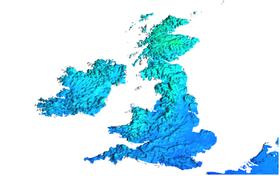
\includegraphics[width=0.3\textwidth]{./images/color_map1.png}
    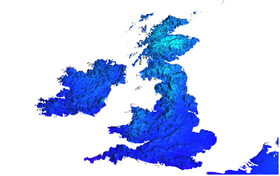
\includegraphics[width=0.3\textwidth]{./images/color_map2.png}
    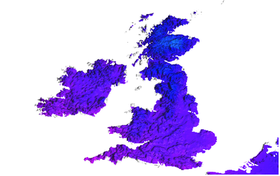
\includegraphics[width=0.3\textwidth]{./images/color_map3.png}
    \caption{Change of color map (temperature)}
    \label{fig:color_map}
    \end{subfigure}
    
    \begin{subfigure}[h]{\textwidth}
    \centering
    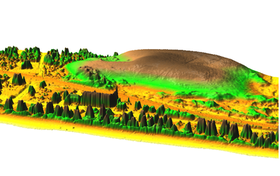
\includegraphics[width=0.3\textwidth]{./images/elevation_map1.png}
    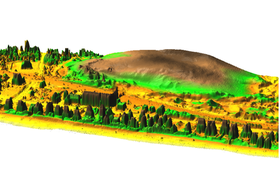
\includegraphics[width=0.3\textwidth]{./images/elevation_map2.png}
    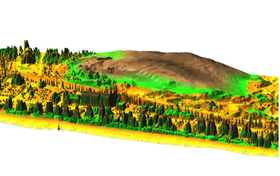
\includegraphics[width=0.3\textwidth]{./images/elevation_map3.png}
    \caption{Change of elevation map (Nags Head area)}
    \label{fig:elevation_map}
    \end{subfigure}
    \caption{Example}
    \label{fig:color_elevation_map}
\end{figure}

        
      
\paragraph{Export}
Animation can be exported either as a sequence of images or an animated gif.
%TODO: add example of ffmpeg command
Sequence of images can be converted to a video file in several ways.
One of the possibilities is to call ffmpeg\footnote{\url{http://ffmpeg.org/}} with the following parameters
      
\begin{footnotesize}
\begin{lstlisting}[style=mybash]
ffmpeg -r 10 -i input_%02d.png -sameq -vcodec mpeg4 output.avi
\end{lstlisting}
\end{footnotesize}
      where \emph{-r} stands for frame rate (frames per second),
      \emph{-i} for input files (requires sequential numbering of files) and
      \emph{vcodec} determines the video encoding.
      The export dialog provides the user with the frame rate, so that he can then create
      a video with the same frame rate%
      \footnote{However, not all video codecs and containers support an arbitrary frame rate.} as in the \at.

      A usual requirement is include some additional text, logo or time stamp in the video.
      The \at supports all these options, moreover the number of these decorations is not limited.
      The placement is specified as the percentage of the image size from the top left corner.
      

\subsection{Support of the \tf}
\label{sec:wx.animation:support}
The \at supports the \tf in several ways. Certain features use the \tf in a more complex way than the others.

The \at accepts space time raster dataset as an input. By the means of the \tf, it determines the maps which are then loaded.
Apart from that, also multiple raster maps are accepted directly.

However, the main difference between displaying a set of maps and a space time dataset is
that the duration of each key frame is given by the given time stamp information.
This is useful when data are collected in irregular intervals.
Then, the key frames do not change e.g.\ every second but at a given moment the frame stays visible for a longer time.
To achieve similar behavior it is necessary to add the frame multiple times, see figure \ref{fig:temporalDifference}.
Concerning temporal data having interval time, there are cases when no data were collected or measured at all.
The \at recognizes such cases and displays a ``no data'' sign in order to make the user aware of the gap in data.

\begin{figure}[ht]
  \centering
\framedInterval{2.5cm}{$X_1$}{(2001, 2002]}%
\framedInterval{5cm}{$X_2$}{(2002, 2004]}%
\framedInterval{2.5cm}{$X_3$}{(2004, 2005]}%

\framedInterval{2.5cm}{$X_1$}{}%
\framedInterval{2.5cm}{$X_2$}{}%
\framedInterval{2.5cm}{$X_2$}{}%
\framedInterval{2.5cm}{$X_3$}{}%

\caption{Difference in animations of temporal data and non-temporal data collected at irregular intervals}
\label{fig:temporalDifference}

\end{figure}

In case of loading more space time datasets the \tf enables to synchronize the animations
even if the temporal datasets are spaced unequally.
Figure \ref{fig:synchronizedAnim}) presents an example of such datasets and the related table
shows the frames displayed at selected time instances.
The concept of temporal granularity and temporal sampling is used to achieve this described behavior.


\begin{figure}[ht]
\centering
\begin{minipage}{10cm}
\framedInterval{75pt}{$X_1$}{}%
\framedInterval{25pt}{$X_2$}{}%
\framedInterval{50pt}{$X_3$}{}%
\framedInterval{100pt}{$X_4$}{}%

\framedInterval{25pt}{$Y_1$}{}%
\framedInterval{100pt}{$Y_2$}{}%
\framedInterval{25pt}{$Y_3$}{}%
\framedInterval{50pt}{$Y_4$}{}%

\vspace{10pt}

\hspace{-3pt}$\uparrow$\hspace{45pt}$\uparrow$\hspace{45pt}$\uparrow$\hspace{93pt}$\uparrow$

\hspace{-3pt}$t_1$\hspace{45pt}$t_2$\hspace{40pt}$t_3$\hspace{90pt}$t_4$
\end{minipage}

\bigskip

\begin{tabular}{lcc}
\toprule
Time & Animation X & Animation Y \\ \midrule
$t_1$ & $X_1$& $Y_1$\\
$t_2$ & $X_1$& $Y_2$\\
$t_3$ & $X_3$& $Y_2$\\
$t_4$ & $X_4$& ---\\\bottomrule
\end{tabular}

\caption{Synchronized animations of space time datasets $X$ and $Y$}
\label{fig:synchronizedAnim}
\end{figure}

Datasets with interval and point time have to be distinguished.
Displaying interval data means to display each map (frame) for the time interval given by its start and end time.
However, point data have no end time. Therefore a different logic must be used to determine when each map should be displayed.
The \at treats point data as interval data where the end time of one map is the start time of the following map.

The time stamp information extracted from the dataset is presented to the user.
The format is given by the \emph{GRASS Datetime Library}. % which url too put here?
The support of other date time formats is planned.


\subsection{Usage}
There are two ways to launch the \at.
First option is to launch it from Layer Manager menu.
If there are any raster maps selected in the Layer Manager, the \at will load these maps automatically.
This simplifies the workflow of analyzing data as it is not necessary to specify maps several times.

Another option, which might appear more natural to many GRASS users,
is to launch the \at as a module from command line. By typing:

\begin{small}
\begin{lstlisting}[style=mybash]
> g.gui.animation
\end{lstlisting}
\end{small}

the \at is launched with no data loaded and the user is supposed to specify maps via the GUI.
Additionally, input data can be specified directly in the command line.
As of any other GRASS module, the parameters of \mod{g.gui.animation} command can be retrieved by typing:

\begin{small}
\begin{lstlisting}[style=mybash]
> g.gui.animation --help

Description:
 Tool for animating a series of GRASS raster maps
 or a space time raster dataset

Usage:
 g.gui.animation [rast=name[,name,...]] [strds=name] [--verbose]
   [--quiet]

Flags:
 --v   Verbose module output
 --q   Quiet module output

Parameters:
   rast   Raster maps to animate
  strds   Space time raster dataset to animate
\end{lstlisting}
\end{small}

The command line interface does not allow the access to complete functionality of the \at.
The reason is that providing all functionality through command line parameters
would result in too complicated parameters.
Moreover, this simple interface should be sufficient for most cases.


\subsection{Implementation}
While \mod{xganim} module was written in wxWidgets using C++ programming language (in GRASS 7),
the \at is written completely in wxPython using Python so that it can be better integrated into the GRASS wxGUI.
It uses \emph{GRASS Python Scripting Library} and \emph{GRASS Python Temporal Library} \cite{grassProgMan},
which is the integral part of the \tf. In the following paragraphs, some of the implementation issues are described.

\subsubsection{Loading data}
It is important to be aware of the fact that animation can consist of hundreds of maps.
Unfortunately, the mechanism of loading raster data in \mod{xganim} could not be simply
rewritten into Python because of performance issues.
Therefore it was necessary to choose a different implementation.

If we try to use the \mod{xganim} implementation, we encounter two main problems.
First, when loading data, the \emph{GRASS Raster Library} functions \cite{grassProgMan} are called.
In Python we could use ctypes to interface these methods,
however these methods can call exit function which causes a sudden end of the program.
This behavior is sufficient for a module but it is not suitable for a long running GUI application.
Secondly, the image representing the raster map is created by setting the color of each pixel sequentially.
For this kind of operation, Python is too slow comparing to C or C++.
This problem can be alleviated by using NumPy\footnote{\url{http://numpy.scipy.org/}},
however that makes the code less readable.

One possible solution is to use the current system used by wxGUI
where the raster maps are rendered into temporary files by module \mod{d.rast}.
However, this method is quite slow mainly because it is necessary to write data to disk and read them afterwards.
Therefore, this method was rejected for the time being.
There have been efforts to improve the rendering implementation%
\footnote{see related ticket \url{http://trac.osgeo.org/grass/ticket/1719}}
and once it is implemented it will not be a problem to change it also in the \at.

Eventually, the raster rendering is done by \mod{r.out.ppm}.
It can send image data to standard output and
thanks to the simplicity of the PPM format (Portable Pixmap Format%
\footnote{\url{http://netpbm.sourceforge.net/doc/ppm.html}}),
the data are directly (without saving to file) converted into the image displayed in the \at.
The advantage of this solution is that the demanding computation is done inside the module, thus in C.
Moreover, if the module fails for any reason, the application is able to handle such situation and continue.
Still, the achieved performance is worse comparing to \mod{xganim}.
This is probably caused by the fact that each call of the module requires not negligible amount of time.
Table \ref{tab:comparisonTime} shows a performance comparison of the described methods.
The time measurement was done on one computer and each number is a sample mean computed from 5 measurements.
To make the measurement more objective, the \mod{xganim} source code was slightly
changed by avoiding reporting messages which would slow the loading down.
The absolute numbers are not as important, however when we compare one with another,
we can see that the difference between the new implementation and the original one is not so significant.
Additionally, there is one important aspect which effects the loading duration
significantly for all implementations\,---\,the size of the map.
If we double the size of the image, we can expect the duration to increase four times.

\begin{table}[h]
  \caption{Time needed for loading a space time raster dataset containing 224 maps (800~$\times$~347~pixels)}
  \label{tab:comparisonTime}
  \centering
    \begin{tabular}{lrr}
    \toprule
    original xganim & 46 s & 100 \%\\
    calling \mod{r.out.ppm} & 51 s & 111 \%\\
    \mod{d.rast} rendering to file (wxGUI) & 67 s & 146\%\\
    \bottomrule

    \end{tabular}
\end{table}




\begin{comment}
244 maps
r.out.ppm
51.177767992
51.0374698639
51.213670969
51.17771101
51.2618360519
========
51.174

66.5165150166
65.1940889359
65.5398728848
72.5624401569
65.7088599205
=====
67.104

46.050000
46.260000
46.260000
46.060000
46.110000
========
46.148
\end{comment}

The images are stored internally as \verb|wx.Bitmap| \cite{wxPythonDoc} objects.
The number of bitmaps is not limited programmatically,
however in reality it is limited by the the size of the bitmaps and available RAM.
This is not an issue for usual animations today.

\subsubsection{Window resizing}
Every application has to react on the change of its frame size.
Unlike \mod{xganim}, the \at is able to resize the displayed images to fit the new frame size.
However, the images are only rescaled, so it produces less quality images.
On the other hand, the rescaled images are sufficient and the advantage is that
the data do not have to be reloaded every time the user resizes the window.
In the application status bar a warning appears to make the user aware of the fact
that the displayed data should be reloaded.

\subsubsection{Specifying the displayed extent}
The displayed extent of the maps is determined by the computational region%
\footnote{This region defines the geographic area (and resolution) in which all raster analyses are done.}.
To change the displayed region, it is necessary to run module \mod{g.region} and then reload data.
At this stage, any interactive zooming would be problematic.
The best option would be to reuse the wxGUI rendering system including zooming in order to avoid code duplication.
Unfortunately, reloading all maps in this way would be more time-consuming.
When the wxGUI rendering system becomes faster
it will hopefully be  possible to reuse this system completely.


\subsubsection{Temporal sampling}
Displaying animation of datasets with unequally spaced intervals or instances is not a simple task.
The \tf which supports the concept of temporal granularity and temporal sampling makes this task feasible.

There are a few computations needed to display the right maps at the right moments.
These steps are the same no matter if there are one or more space time datasets.
The first step is to get the time granularity.
The second step is the sampling of each dataset by the granularity using temporal relation \emph{start}.
This way we get all needed information about the time intervals (or instances) and the names of the maps.
The \at then puts all of this information together.

Table \ref{tab:exampleOfSamplingImpl} shows the result of temporal sampling of two sample space time datasets.
As we can see, the temporal granularity of the dataset $X$ (1 month) differs from the granularity of dataset $Y$ (2 months).
The common granularity (1 month) is in this case easy to compute.
This granularity is then used to sample both datasets (table \ref{tab:exampleOfSamplingImpl-2}).


\begin{table}
 \centering
\caption{Example of two space time datasets $X$ and $Y$ and the their sampling by temporal granularity 1 month.}
\label{tab:exampleOfSamplingImpl}
\begin{subtable}{0.4\textwidth}
    \centering
    \caption{List of maps and valid time intervals}
    \begin{tabular}{lll}
    \toprule
    $X$ & start time & end time \\
    \midrule
    $X_1$ & 2001-02-01 & 2001-03-01\\
    $X_2$ & 2001-03-01 & 2001-06-01\\
    $X_3$ & 2001-07-01 & 2001-10-01\\
    $X_4$ & 2001-10-01 & 2001-12-01\\
    \bottomrule
    \end{tabular}

    \vspace{20pt}
    \begin{tabular}{lll}
    \toprule
    $Y$ & start time & end time \\
    \midrule
    $Y_1$ & 2001-01-01 & 2001-03-01\\
    $Y_2$ & 2001-05-01 & 2001-07-01\\
    $Y_3$ & 2001-07-01 & 2001-09-01\\
    \bottomrule
    \end{tabular}
\end{subtable}
\quad
\begin{subtable}{0.4\textwidth}
\centering
\caption{Result of temporal sampling with granularity 1 month}
\label{tab:exampleOfSamplingImpl-2}
\begin{tabular}{llll}
\toprule
 $X$ & $Y$ & start time & end time \\\midrule
--- & $Y_1$ & 2001-01-01 & 2001-02-01\\
$X_1$& $Y_2$ & 2001-02-01 & 2001-03-01\\
$X_2$& --- & 2001-03-01 & 2001-04-01\\
$X_2$& --- & 2001-04-01 & 2001-05-01\\
$X_2$& $Y_2$ & 2001-05-01 & 2001-06-01\\
--- & $Y_2$ & 2001-06-01 & 2001-07-01\\
$X_3$& $Y_3$ & 2001-07-01 & 2001-08-01\\
$X_3$ &$Y_3$ & 2001-08-01 & 2001-09-01\\
$X_3$ & --- & 2001-09-01 & 2001-10-01\\
$X_4$& --- & 2001-10-01 & 2001-11-01\\
$X_4$ & --- & 2001-11-01 & 2001-12-01\\
\bottomrule
\end{tabular}
\end{subtable}

\end{table}

\subsubsection{Animation}
Animation basically means to display a sequence of images in the given time instances.
Crucial is to determine \emph{which} frame (map) and \emph{when} to display.
We first discuss the \emph{when}  and then the \emph{which} question.


The original \mod{xganim} implementation of the animation is rather primitive.
The events are emitted when system becomes idle which the programmer is not able to affect.
Moreover, the delay between two successive frames is done by a for loop
and to change the speed of the animation the number of loops is increased or decreased.
Therefore the default speed of the animation on the current computers is much more faster than it used to be ten years ago.

The \at implementation uses timer events (class wx.Timer provided by wxPython) to achieve regular time intervals between two frames.
The interval between two successive events is specified by the programmer according to what the user requires.
In case of space time datasets animation, the user specifies how long
should a chosen time unit\footnote{units of time supported by the \tf, section \ref{sec:absoluteVsRelative}}
last (in milliseconds).

For each dataset, there is a separate object which controls the animation.
These animation objects receive the timer events and determine
which frame to display according to the result of the temporal sampling explained above.
The timer interval represents the temporal granularity of the datasets.
Therefore, each map is displayed exactly at the right moment.

When the interval of a map takes more than one temporal granularity, internally, there is no redraw.



\subsubsection{Checking compatibility of data}
During the development it was necessary to decide which data are compatible and can be animated together.
Several combinations are possible.
\begin{description}
  \item[Space time dataset $\times$ multiple maps]
  This combination is allowed granted that the number of maps matches the number of maps in the dataset.
  Then, the animation behaves as if there was no temporal information.

  \item[Space time datasets with absolute $\times$ relative time]
  This case is not allowed because there is no obvious way to convert one type to another.

  \item[Space time datasets with interval $\times$ point time]
  This combination is allowed, however it might not behave as user expects.
  Therefore, there is a warning to make the user aware of this fact.
 \end{description}
 
In general, it is better to use data which are fully compatible to avoid confusion.
The \at always checks the user input and in the case it recognizes an incompatibility, it reports it to the user.


\subsubsection{3D view animation}
\label{sec:3dViewAnimation}
Images for 3D view animation must be first rendered by module \mod{r.nviz.image} \cite{grassUserMan}.
The rendering is more time-consuming than loading raster maps for the 2D view,
however this does not affect the speed of the animation itself.

3D view animation requires to specify additional input data.
Beside the maps (either multiple maps or space time dataset), the user is asked for a \emph{workspace file}%
\footnote{Workspace file is XML file storing the state of the wxGUI application (e.g.\ loaded layers, displayed extent).}.
The workspace file has to be created during a GRASS wxGUI session with active 3D view,
so that it can provide information about the 3D view state. After parsing this file, a command for \mod{m.nviz.image}
is created.
Additionally, the user chooses which parameter to animate.
Typically, it is either \emph{elevation\_map} or \emph{color\_map}
(see the difference between figures \ref{fig:color_map} and \ref{fig:elevation_map}),
although we can animate points or lines, too.

\subsection{Future development}
\begin{itemize}
  \item loading more layers
  \item add where to determine time interval
  \item add legend
  \item better support of formats
  \item 
\end{itemize}



\section{Timeline tool}
Timeline Tool is an interactive application based on wxPython and Python plotting library matplotlib \cite{matplotlib} which allows
the user of the \tf to visualize space time datasets' metadata, especially temporal and spatial extents.

\subsection{Features}
The main purpose of this tool is illustrated by the figure \ref{fig:timeline1}
which is the output plot generated by the tool.

The x-axis represents time and the space time datasets are located on y-axis.
This simple plot gives an immediate overview of the datasets' temporal extent.

Furthermore, it shows also other characteristics of the datasets.
Interval and point datasets are distinguished by different symbols (points and bars)
which is easily and intuitively understandable.
Datasets with relative and absolute time can be recognized by different x-axis tick labels (date/time format vs. integer).

Also, invalid topology of a dataset is visualized.
Invalid topology basically means overlaying intervals or points
which can be easily represented by using semi-transparency to draw plot.
As a result, overlaying intervals are darker
which allows to recognize them (see figure \ref{fig:timeline1}, red dataset topol\_abs8).

\begin{figure}[ht!]
  \centering
  \begin{subfigure}[ht]{\textwidth}
  \centering
  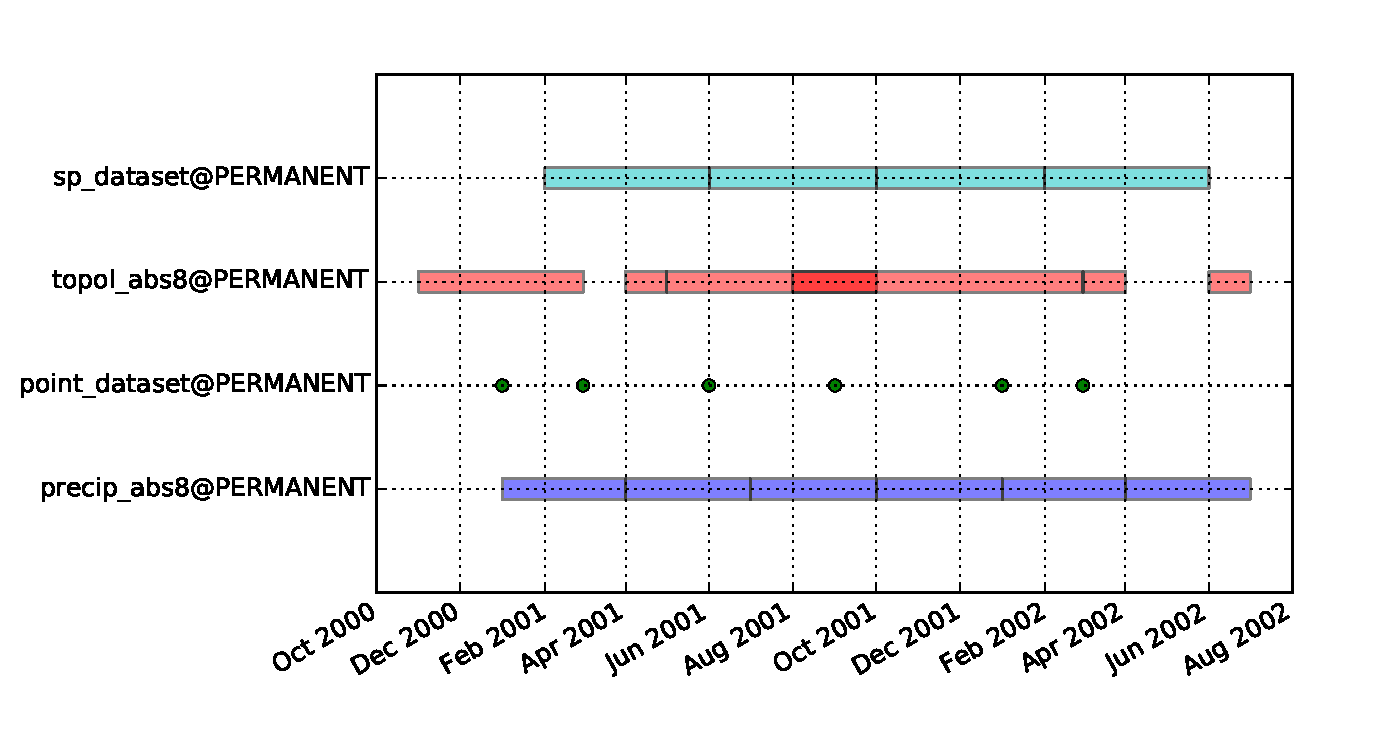
\includegraphics[width=0.8\textwidth]{./images/timeline1.pdf}
  \caption{temporal extents}
  \label{fig:timeline1}
  \end{subfigure}

  \begin{subfigure}[ht]{\textwidth}
  \centering
  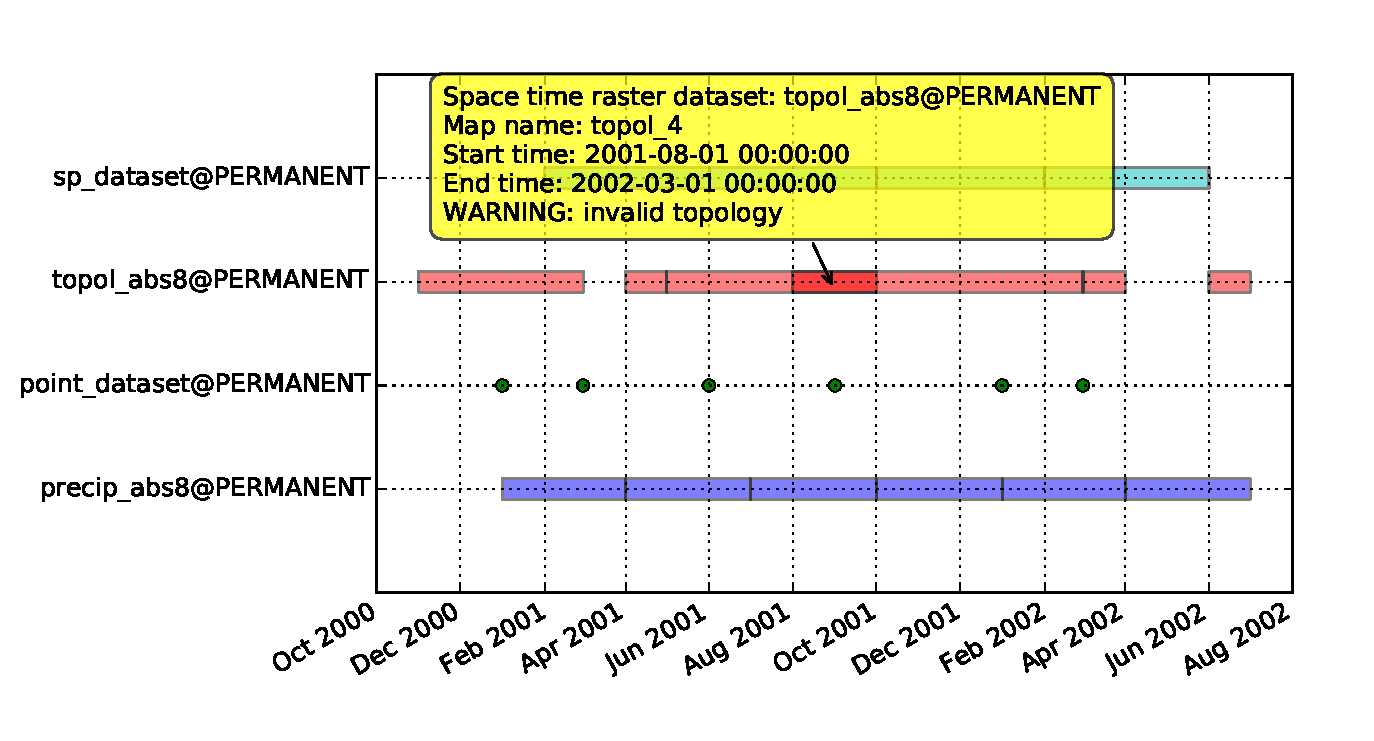
\includegraphics[width=0.8\textwidth]{./images/timeline3.pdf}
  \caption{annotation}
  \label{fig:timeline3}
  \end{subfigure}
%   
\caption{Timeline Tool: 2D plot of datasets' extents}
\label{fig:timeline}
\end{figure}

Other metadata can be displayed by clicking on the plotted dataset.
An annotation bubble appears showing basic information about the dataset and the selected map (figure \ref{fig:timeline3}).
It also warns about invalid topology of the dataset.


Not only temporal extent but also spatial extent can be visualized by using matplolib extension mplot3d.
The 3D plot is a space time cube where x- and y-axis represent the spatial part and the z-axis represents time (figure \ref{fig:timeline2}).

\begin{figure}[ht!]
  \centering
  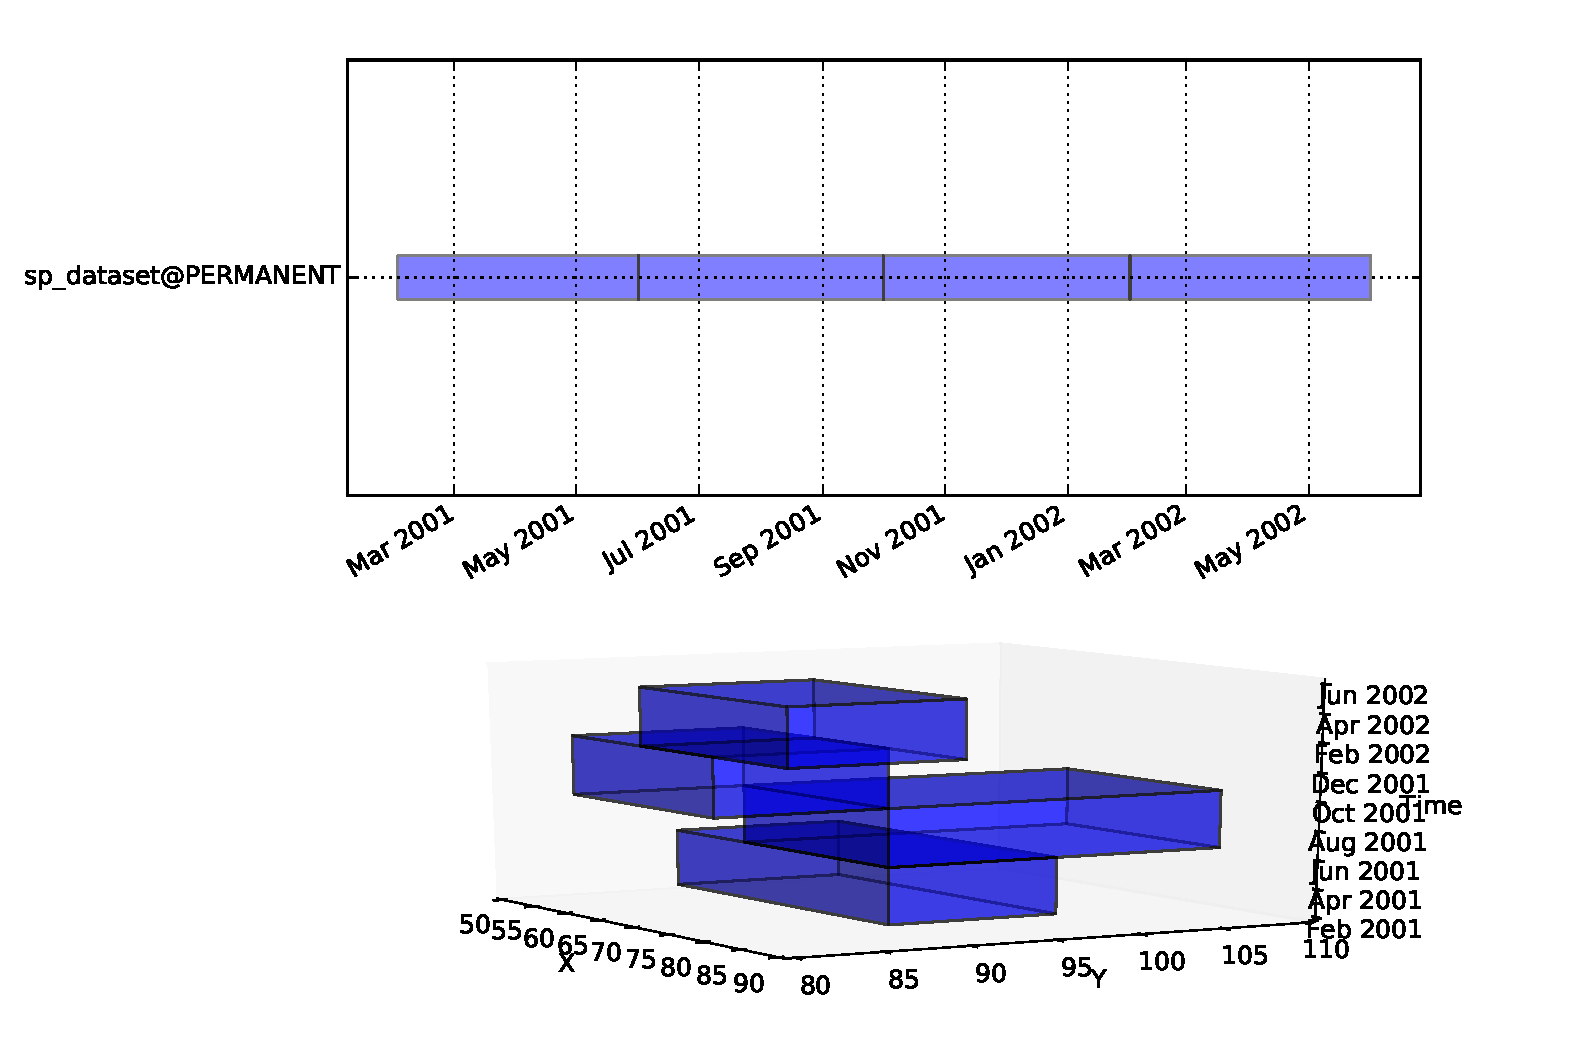
\includegraphics[width=0.8\textwidth]{./images/timeline2.pdf}
  \caption{Timeline Tool: spatial and temporal extents}
  \label{fig:timeline2}
\end{figure}

In order to better explore plotted data, the application allows to zoom,
pan (and in the case of the 3D plot also rotate) the plot.
This functionality is provided by matplotlib's navigation toolbar which is a great advantage both for programmers and users.
Moreover, this toolbar offers to export figure to various raster and vector formats.

\subsection{Implementation}
To achieve nice and interactive plots integrated into wxPython application, matplotlib was chosen as a best option.
Although matplotlib is not a required dependency for GRASS~7,
users often have this library already installed because of its usefulness and capabilities.
Another considered option was a wxPython module wx.lib.plot.
Despite the advantage that it is already a part of wxPython and thus, no other dependency would be required,
it lacks the ability to display time stamps as axis tick labels. This crucial functionality is available in matplotlib.

The Timeline Tool embeds matplotlib into wxPython program by using WXAgg backend.
This enables to integrate the figure canvas and the navigation toolbar
which provides zooming, panning and export functionality.
Beside this toolbar, the Timeline Tool has additional wxPython widgets to control user input.

Matplotlib is a Python library which is an active project and new versions are released approximately two times a year.
Unfortunately, this means that new versions can have different API and new functions unavailable in older versions.
This makes it hard or even impossible to provide the same functionality for all versions.
The Timeline Tool suffers from this problem, too.
The 3D functionality is not available for matplotlib versions older than 1.0.0 (January 2011)
because of slightly different API, the inability to easily combine 2D and 3D subplots in one figure
and the lack of support for alpha drawing.
The Timeline Tool was tested both with an older version 0.99.1 (available for Ubuntu 10.04) and the latest version 1.1.1.

The 3D functionality of matplotlib is still in development and there are many known problems%
\footnote{\url{http://matplotlib.org/mpl_toolkits/mplot3d/faq.html}}.
These issues will be hopefully fixed in future versions of matplotlib.
% Therefore, the Timeline Tool's 3D view is m


\subsection{Usage}
The Timeplot Tool can be launched as any other GRASS module.
For displaying help, choose one of the following options:
\begin{small}
\begin{lstlisting}[style=mybash]
> g.manual entry=g.gui.timeline # opens manual page in a browser
\end{lstlisting}
\end{small}

\begin{small}
\begin{lstlisting}[style=mybash]
> g.gui.timeline --help

Description:
 Allows to compare temporal datasets
 by displaying their temporal extents in a plot.

Usage:
 g.gui.timeline [-3] [inputs=name[,name,...]] [--verbose] [--quiet]

Flags:
  -3   Show also 3D plot of spatio-temporal extents
 --v   Verbose module output
 --q   Quiet module output

Parameters:
  inputs   Name of the input space time datasets

\end{lstlisting}
\end{small}

\subsection{Future development}
Next development will focus on the following points:
\begin{itemize}
  \item highlighting individual maps, which should be synchronized in 2D and 3D
  \item support for datasets with `mixed' time (time instances and intervals together in one dataset)
  \item user settings\,---\,colors, date formatting
\end{itemize}
In the future, such tool could be integrated into any application processing temporal data
and then, it could be used as a control widget.



\section{\ms}
\ms is a tool which allows the user to interactively compare two raster maps
of the same area by revealing different parts of the raster maps.
It is useful for comparing raster maps from different time periods.
Although \ms does not use the \tf, as there is no particular application for it,
thanks to its capabilities we can regard it as an useful tool for exploring spatio-temporal data.

An example of usage is presented on the manual page \cite{grassUserMan} of the \ms.
\begin{figure}[h!]
  \centering
  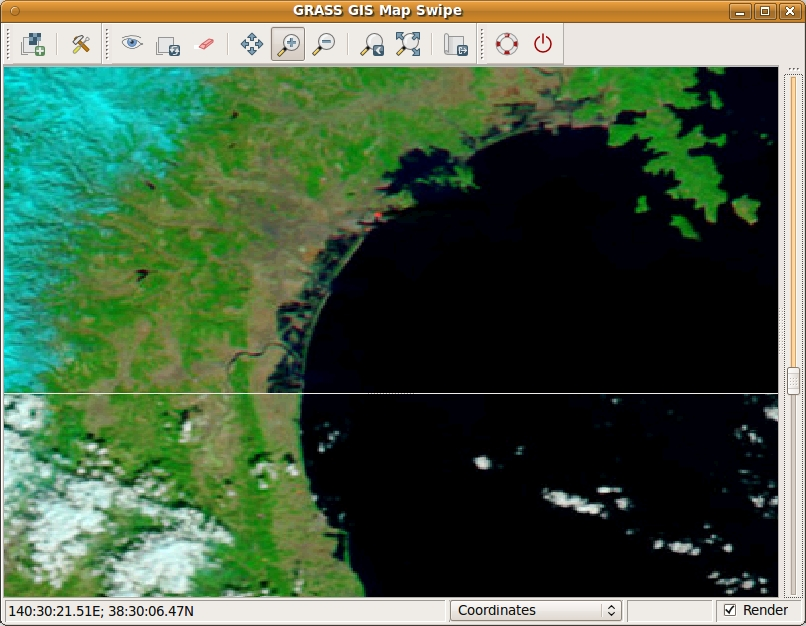
\includegraphics[width=0.8\textwidth]{./images/mapswipe_tsunami.jpeg}
  \caption{Pre and post disaster images of the tsunami in Japan in 2011.
  The upper MODIS image taken on February 26, 2011, shows the coastline under normal conditions
  while the lower MODIS image on March 13, 2011, shows a clear view of tsunami flooding along the coastline.
  Water, black and dark blue in these false-color images, still covers the ground as much as five kilometers
  (three miles) from the coast. Source: Earth Observatory/NASA}
\end{figure}


\subsection{Features}
Map Swipe allows to:
\begin{itemize}
    \item switch orientation of the swipe line (horizontal or vertical)
    \item zooming, panning

\end{itemize}

    
\subsection{Usage}
automatically load maps when opening Map Swipe with two selected raster maps in Layer Manager












\newpage
\clearpage
\printbibliography

\end{document}
